
\chapter{Theoretical background}\label{chap:theory}

\section{FEST-Swing}\label{sec:fest-swing}

FEST (Fixtures for Easy Software Testing) is a collection of libraries whose mission is to simplify software testing. It is composed of various modules, which can be used with TestNG or JUnit. The most significant module is the FEST-Swing module.

The Swing module provides a simple and intuitive API for functional testing of Swing user interfaces, resulting in tests that are compact, easy to write, and read like a specification. Tests written using FEST-Swing are also robust. FEST simulates actual user gestures at the operating system level, ensuring that the application will behave correctly in front of the user. It also provides a reliable mechanism for GUI component lookup that ensures that changes in the GUI's layout or look-and-feel will not break the tests \cite{FESTMain}.

\subsection{Introduction}

A FEST-Swing test is testing either individual frames (the building blocks of a UI), or entire Swing applications or Applets. FEST simulates actual user gestures (mouse movements, keys presses) at the operating system level, ensuring that during the application will behave in the same way as in the front of the user. It uses AWT Robot, which generates events in the platform's native input queue. Thus, the test needs to create the components and make them visible on the screen, and the tests will actually moves the mouse cursor, and not just only generates mouse move events.

\subsection{Architecture}

FEST Swing's component fixture architecture is separated into several layers (from bottom to top):
\begin{enumerate}
\item BasicRobot: Simulates a user interacting with a mouse and keyboard. It uses the AWT Robot to generate native input events.
\item Component driver: This layer does all the ``heavy lifting.'' All interaction with a GUI component is done in this layer. It knows how to simulate events and check the state of a specific GUI component. For example, JComboBoxDriver knows how to simulate a user using a JComboBox (selecting a particular element) and how to verify the state of it (which element should be selected.)
\item Component fixture: This layer sits on top of the driver. It provides a fluent interface to that and makes the API easier to write and read. Users of FEST write their GUI tests using fixtures, not drivers. There is one fixture per Swing component, and each fixture has the same name as the Swing component they can handle ending with ``Fixture.'' For example, a JButtonFixture knows how to simulate user interaction and verify state of a JButton. Fixtures can be considered the ``user interface'' of the FEST-Swing library.
\end{enumerate}

The architecture also supports extensions, so developers of application using custom Swing components can write their own fixtures and component drivers.

\subsection{Example}

Writers of GUI tests need to use the fixtures located in the package org.fest.swing.fixture. These fixtures provide specific methods to simulate user interaction with a GUI component and they provide assertion methods that verify the state of the GUI component. Although it is possible to work with the FEST BasicRobot directly, the BasicRobot is too low-level and requires considerably more code than the fixtures.

As a concrete example, let us consider a very simple JFrame that contains a JTextField, a JLabel and a JButton, and component has its unique name. The expected behavior of this GUI is the following: when user clicks on the JButton, the text of the JTextField should be copied to the JLabel. (Figure \ref{fig:example_jframe}) 

\begin{figure}[h!] \label{fig:example_jframe}  
  \centering
    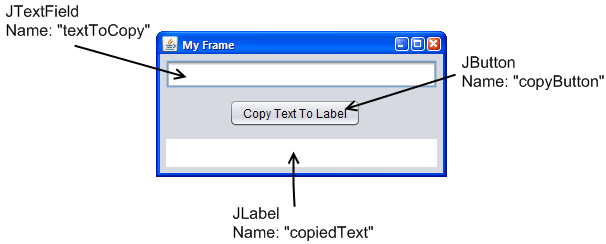
\includegraphics[width=0.6\textwidth]{images/example_jframe.png}
  \caption{A very simple JFrame that contains a JTextField, a JLabel and a JButton.}
\end{figure}

To the frame, the test's setup method needs to create the frame (in the EDT, delegating it with GuiActionRunner), create a fixture for it, and make it visible (Figure \ref{fig:example_setup_method}).

\begin{figure}[h!] \label{fig:example_setup_method}
\begin{lstlisting}
protected def onSetUp() : Unit = {
    val frame : MyFrame = GuiActionRunner.execute(new GuiQuery[MyFrame] {
        protected def executeInEDT() : MyFrame = new MyFrame
    })
    window = new FrameFixture(robot, frame)
    window.show() // shows the frame to test
}
\end{lstlisting}
\caption{The setup method creating the frame and the fixture, and making it visible.}
\end{figure}

The test method can use the fixture to simulate a user interacting with a GUI in order to verify that such GUI behaves as we expect. The user interactions and the assertions in the test are fluent and simple. The method looks up the UI components by their unique names. (Figure \ref{fig:example_test_method})

\begin{figure}[h!] \label{fig:example_test_method}
\begin{lstlisting}
@Test 
def shouldCopyTextInLabelWhenClickingButton : Unit = {
    window.textBox("textToCopy").enterText("Some random text")
    window.button("copyButton").click()
    window.label("copiedText").requireText("Some random text")
}
\end{lstlisting}
\caption{The test method.}
\end{figure}

It is important to mention that besides testing individual components that build up an application, FEST-Swing also supports testing entire applications. In such cases, the first tests starts up the application with ApplicationLauncher that understands how to launch an application using its main method. Once the application is started, the test just needs to find the application's main window.

\subsection{Threading model}

The documentation of FEST-Swing strongly advises to respect Swing's threading rules \cite{OracleSwingThreading} both in the tests and in the tested application (this remains only an advice because Swing itself does not enforce thread safety). In short, the cardinal rule is the following: creation and access (both read and write) of Swing components should be done in the Event Dispatch Thread (EDT.) Since JUnit and TestNG tests do not run on the EDT, creation and any direct access in the tests to Swing components should be delegated to EDT via the utility class GuiActionRunner (or via other tools).

To ensure that the threading rules are respected throughout the tests and the tested application, FEST Swing provides the class FailOnThreadViolationRepaintManager. It forces a test failure if access to Swing components is not performed on the EDT. However, it only detects component creation and writing, and is unable to detect read operations (component creation and writing triggers repaint events, but read does not).

\subsection{Limitations}\label{sec:fest-swing-limitations}

Because FEST-Swing is actually simulating user interaction, it needs an environment very similar to actual user environments: the tested application needs to be active and in focus, and needs to move the mouse. Therefore, that machine that the tests run on cannot be used for the entire duration of the tests. In addition, the tests probably fail whenever another applications unexpectedly gets the focus and covers the application's window (the mouse no longer clicks the correct application). This can become a burden because UI tests, by their nature, can take a significant amount of time to execute and especially when using agile development methods, it is preferable to run them frequently.

Because of this, it is common to delegate the tests to Continuous Integration (CI) systems (e.g. Hudson/Jenkins, TeamCity etc.) When the CI platform is based Linux, BSD or UNIX-style operating systems, it is common that the server does not even have the X Window system, running applications with UI impossible. For this case, Xvfb offers a simple and straightforward solution \cite{FESTxvfb}.

However, if the target platform is Windows, there are a whole set of issues, and the known solutions are problematic, and are very complicated and time consuming to setup. \cite{HudsonUnderWindows} \cite{Cacio_Tta_FEST}

To overcome all of these limitations, OpenJDK's project Caciocavallo can be used \cite{Cacio_Tta_FEST} to provide a graphics stack for the Java VM that is completely independent from the environment, eliminating any need for platform-dependent setup for CI systems. It renders everything into a virtual screen (which is simply a BufferedImage object), and is driven solely by AWT Robot events. However, this also has its own limitations; the most important being that drag-and-drop \cite{IntroDnD} is unsupported, thus it needs certain workarounds (see \fullref{sec:simulated-dnd}).

\section{User Action and Adapter design pattern}\label{sec:user-actions-adapters}

The users using an application with a UI typically interact with it by executing a series of operations that change the application's state. These operations might themselves be consisting of multiple operations of the UI components, changing the UI's state and, indirectly, changing the application's internal state. UI test simulating the users can incorporate in their architecture the concept of separation: the tests can interact with a user action layer (consisting of the actions the user can do with the application), and the user actions can interact with an adapter layer that itself interacts with the UI components (e.g. by using FEST-Swing).

The same separation applies to the tests' assertions: the tests assert the application's state through the user actions, and the user actions assert the UI's state, and thus, indirectly, assert the application's internal state.

\subsection{Adapters}

The adapters understand how to execute operations on the application by using the UI components. 

For example, to create a new text file in an editor application supporting multiple types of files, the user typically needs to click on the File menu, then on the menu item New, and then on the sub-menu-item Text file. The combinations are usually limited (the submenu-item cannot be clicked without clicking the menu item first), and sometimes require some checking (if the File menu is already visible for whatever reason, the test should not click it again because that would only close the menu).

These operations come from the functional specification of the application, and their implementation details are only dependent on the UI design. These operations can be structured into adapters, where each logically bound component group can have a corresponding Adapter class (e.g. FileMenuAdapter), where the methods are the operations (e.g. FileMenuAdapter\#clickNewTextFile()). The adapter class can have a fixture for each Swing component, and the methods can directly interact with them.

This approach also leads to tests that are more resistant to UI changes, requiring less code change for each UI design change. For example, if the in the UI design of the above text editor the Text file menu item is moved directly into the File menu under the name New text file, only the appropriate adapter class needs to be modified, while all the tests using this operation are left unchanged. Whereas, if the code using the fixtures and clicking on the menu items was present in all the tests, such a change would need all the tests to be changed.

\subsection {User actions}

The user actions understand how to execute operations of the application by using the adapters. 

For example, let us consider a case where the user wants to save the file in the current editor of an editor application with a new name. The user needs to click the Save as menu item, resulting in the appearance of a browser dialog. After that, he needs to enter the new file name into a text box, and then needs to click the OK button of the dialog, and finally wait for the dialog to disappear. In this case, the file menu can have an adapter; the file browser dialog can have an adapter; and using both of them in the same time in a given way can represent a user action. For example, the user actions related to the current edited document can be grouped into a user action class (EditorUserAction), and where the methods are the user actions (EditorUserAction.saveAs(newFileName)).

\section{Scala}

Scala is a general-purpose object-oriented and functional programming language that runs on the top of the JVM. Besides supporting all the standard OOP concepts (classes, inheritance, encapsulation etc.), Scala has full support for functional programming (including currying, pattern matching, algebraic data types, tail recursion, lazy initialization, immutability etc.) Scala has a unified type system (meaning that there is no distinction between primitives and classes), supports anonymous types, operator overloading, optional parameters, named parameters, string interpolation, and so on. All these put together, Scala enables a programmer to develop very concise and small programs.

Scala and Java have commons roots. Scala's main designer and developer, Martin Odersky, is also known for developing the programming language \emph{Generic Java} (which, with the addition of wildcards, was integrated into \emph{Java 5}), and for the development of the current generation of \emph{javac}, the Java Compiler. Many of Scala's syntax elements were inspired by Java (e.g. the imperative control structures, operators). Many of Scala's design decisions were inspired by criticism over the shortcomings of Java.

The Scala source code is compiled to Java bytecode, so the resulting executable runs on the Java virtual machine. Existing Java libraries can be directly used in Scala code, and vice versa. 

\subsection{General syntax}

Scala uses the curly-brace syntax reminiscent of the C programming language. A simple hello-world program looks like the following:

\begin{lstlisting}
object HelloWorldApp extends App {
  println("Hello, world!")
}
\end{lstlisting}

Note that contrary to a hello-world application in Java, there is no class declaration and no static main method declaration; instead, a singleton object is created with the keyword \texttt{object} whose body consists of the application. In order to be compatible with the JVM, a class with a method \texttt{static void main(String[])} is generated.

A local variable or a field is declared with the keyword \texttt{val} or \texttt{var}. The keyword \texttt{val} is used for variables that are initialized only once and never change their value, and the keyword \texttt{var} is used for variables whose value changes during the execution. For example:

\begin{lstlisting}
val end = 100 // constant
var sum = 0  // variable, changed in the loop below
for (i <- 1 to end) {
  sum += i
}
println(s"The sum of numbers between 1 and $end is $sum")
\end{lstlisting}

The following example defines a method that calculates the below expression:

\[
f(x) = 
  \begin{cases}
    \frac{1}{x^2} & \text{if } x \neq 0 \\
    0 & \text{if } x = 0
  \end{cases}
\]

\begin{lstlisting}
def f(x: Double): Double = {
  if (x != 0) {
    val square: Double = x*x
    return 1 / square 
  } else {
    return 0
  }
}
\end{lstlisting}

Note that the type \emph{follows} a name (as in Pascal) rather than \emph{preceeds} a name (as in C or Java). This, together with the mandatory initialization of variables, enables \emph{type inference} to take place, making type declarations optional for variable declarations, fields, and even (non-abstract) methods. In the above example, all the type declarations, with the exception of the parameter \texttt{x}, can be ommited. The following code is equivalent:
\begin{lstlisting}
def f(x: Double) = {
  if (x != 0) {
    val square = x*x
    1 / square 
  } else 0
}
\end{lstlisting}

It is also possible to omit the return statement. This is because in Scala everything is an expression and thus has a value. The value of a block (delimited by the curly braces \texttt{\{\dots\}}), is equal to the value of the \emph{last} expression inside the block, and value of the statement \texttt{if (condition) <then-block> else <else-block>} statement is equal to either the value of the ``then-block'' block or the ``else-block'' block, depending on the condition. In Scala code, return statements are typically used only to control the execution flow of a method.

\subsection{Type system}

\subsubsection{Classes}

A class is declared in the following way:

\begin{lstlisting}
class C[typeParams](classParams) extends Superclass with Trait {
  definitions
}
\end{lstlisting}

With the exception of the class name, everything can be ommitted. A class may extend (or \emph{mix in}) multiple traits (which are similar to Java interfaces and abstract classes). The class parameters are Scala's equivalent of Java's constructor parameters.

A class can be instantiated with the \texttt{new} operator, similar to Java.

\subsubsection{Singleton objects and companion objects}

With the use of the \texttt{object} keyword, it is possible to declare a singleton object:
\begin{lstlisting}
object O extends Superclass with Trait {
  definitions
}
\end{lstlisting}

Package-level singleton objects can define fields and methods that are accessible throughout the entire application, and thus are similar to Java's static fields and methods. In addition to that, a singleton object can extend a class or traits,  which is not directly possible in Java.

A \emph{companion object} is a singleton object that has the same name as a class defined in the same scope. For example:

\begin{lstlisting}
class Complex(val r: Double, val i: Double) {
  def +(c: Complex): Complex = \dots
}
object Complex {
  val zero = new Complex(0, 0)
  val one =  new Complex(1, 0)
  val i = new Complex(0, 1)
  def apply(r: Double = 0, i: Double = 0) = new Complex(r, i)
}

val c1 = Complex(2) // calls Complex.apply(2)
val c2 = Complex(2, -1) // calls Complex.apply(2, 3)
val c3 = Complex() // calls Complex.apply(0, 0)
val c4 = Complex(i = 1) // calls Complex.apply(0, 1)
val c5 = new Complex(2, 3)
val c6 = Complex.one + Complex.i
\end{lstlisting}

This is in direct parallel with a class in Java having both static and instance members: the members defined in the companion object correspond to the the static members, and the members defined in the class correspond to the intance members. Note that this is also actually how classes with companion objects are implemented in Scala (the compiler generates only one class with static and instance members).

The above example uses Scala's equivalent of overloading the method call operator \texttt{()}: the expression \texttt{a(x)} is equivalent to \texttt{a.apply(x)} where \texttt{a} is an object of a type that defines the method \texttt{apply}.

\subsubsection{Traits}

Traits are Scala's replacement for Java interfaces. In Java versions prior to 8, interfaces are highly restricted, able to contain only abstract method declarations. This leads to difficulties with convenience methods (the same methods must be reimplemented in each implementing class), and to inability to extend an interface without breaking compatibility (issue for published libraries). Traits in Scala are similar to an abstract class in Java: besides defining abstract methods (just as an interface), they can provide implementations for methods, and can even have fields. A trait can extend an extend one or more other traits, and even classes. The only limitation of a trait a trait cannot have parameters (constructors).

\subsection{Syntactic flexibility}
Scala has significantly more flexible syntax when compared to Java. This includes:
\begin{itemize}

\item Semicolons are unnecessary for statements that are otherwise delimited by new lines. Semicolons are used only when more than one statement is present on a line.

\item Any method can be used as an infix operator. For example, \texttt{"\%d apples".format(count)} is equivalent to \texttt{"\% apples" format count}. This is in fact how operator overloading is possible: since method names can consist of any characters, it is possible to define a method with a symbol in its name, and then use the method as an infix operator. For example: 

\begin{lstlisting}
class Complex(val r: Double, val i: Double) {
  def +(c: Complex) = new Complex(r + c.r, i + c.i)
  def multiplyBy(c: Complex) = \dots
}
val a = new Complex(1, 2)
val b = new Complex(3, -1)
val sum1 = a + b // sum1 and sum2 are equivalent
val sum2 = a.+(b)
val prod1 = a multiplyBy b // prod1 and prod2 are equivalent
val prod2 = a.multiplyBy(b)
\end{lstlisting}

\item Possible to overload the function call operator --- methods \texttt{apply} and \texttt{update} have shorts forms similar to function calls. For example, where \texttt{a} is a class instance or singleton object, \texttt{a()} is equivalent to \texttt{a.apply()}. The method can parameters as well, e.g. \texttt{a(42)} is equivalent to \texttt{a.apply(42)}. The method \texttt{update} has an equivalent assignment-like syntax: \texttt{a() = 42} is equivalent to \texttt{a.update(42)}, and \texttt{a(4) = 2} is equivalent to \texttt{a.update(4, 2)}.

\item Scala supports the Uniform Access Principle: it is transparent to the user of a class whether a property of an object is implemented by directly using a field or by using getter-setter methods. In Scala, public \texttt{val} or \texttt{var} members can be overridden by getter-setter methods and vice-versa. This is in contrary to Java, where explicit getter-setter methods are required and the public fields exposed by a class cannot be overridden by getter-setter methods in subclasses. For example:

\begin{lstlisting}
trait Person {
  var name: String // abstract
}

class Student extends Person {
  private var _name: String
  def name = _name
  def name_=(newName: String) { _name = newName }
}

val p: Person = new Student
p.name = "Foo Bar"
println(p.name)
\end{lstlisting}

\item Scala supports the definition of constructs that are similar to language structures. For example:
\begin{lstlisting}
def safe(f: => Unit) {
  try {
    f()
  } catch {
    case e: Throwable => e.printStackTrace()
  }
}

safe {
  println("This block never throws exceptions")
}
\end{lstlisting}

In the above example, the method call parenthesis were omitted, and the block was automatically converted to an argument of type \texttt{=> Unit} which represents nullary functions returning Unit (equivalent of the Java type \texttt{void}).

\end{itemize}

This syntactic flexibility allows domain-specific languages to be defined in Scala without the need to extend the compiler. For example, the library \emph{Scala-react} defines a custom control-flow language with the use of higher-order functions, by using extensively using \texttt{apply} and \texttt{update} methods, and by using infix method call syntax for operator methods.

\subsubsection{immutability}

\subsubsection{Implicit parameters}

\subsection{Tail recursion}

\subsection{Functions as types}
\subsubsection{higher order functions}
\subsubsection{partial functions}

\subsection{Currying}

\subsection{Standard functional elements}

\subsection{Algebraic data types and pattern matching}

\subsubsection{tuples}

\subsection{Delimited continuations}




\section{Scala-swing}

Scala-swing is a UI library written in Scala that wraps the Java Swing components with the purpose of providing a simpler, more straightforward and typesafe interface that is more natural to use in Scala. It is meant to be sufficiently close to the Java Swing to appeal to Java programmers with existing Swing experience.\cite{ScalaSwing} The library diverges significantly from Java Swing only on parts that are considered as bad design decisions of Java Swing.

The library provides lightweight wrappers around Swing components, maintaining their functionality and hierarchy, reimplementing them in Scala-like terms (using Scala properties instead of getter/setter methods, using enumerations instead of magic constants, and providing a typesafe API for objects like JList). The main divergences are the following:
\begin{itemize}
\item In Java Swing all components are also containers. This doesn't make sense for a number of components (e.g. TextField, CheckBox, Button etc.) This is likely to be because of the lack of multiple inheritance in Java. Scala-swing uses the \emph{trait} \texttt{Container}.

\item Layout managers and panels are coupled, though they are decoupled in Java Swing. Scala-swing offers a straightforward, typesafe API for the standard Swing layout managers in the form of a panel class for each layout (e.g. \texttt{BorderPanel} for a \texttt{JPanel} with \texttt{BorderLayout}).

\item The event mechanism is completely reworked around the concept of publishers and reactors. This offers a more homogeneous API for event management than what Java Swing offers.
\end{itemize}

\section{Scala CPS Plugin}

Delimited continuations are a versatile programming tool. Their most important use is based on their ability to suspend and resume sequential code paths in a controlled way. The Scala CPS plugin is a compiler plugin that enables the programmer to have delimited continuations in direct-style code, without much syntactic overhead. This is implemented by the plugin selectively transforming the source code in compile time, driven by annotations and other structures placed into the code by the programmer. Multiple variants of delimited continuations have been described in the literature, and the Scala CPS plugin implements the so-called Danvy and Filinski model, with two primitive operations, \texttt{shift} and \texttt{reset}.

A delimited continuation embodies a certain part of the program. When invoking a delimited continuation, the control returned to the caller, and it may also return a value. Inside the continuation, at any point the current fragment of the call stack starting from the delimiting block can be saved to be later reused (possibly multiple times), or discarded. This control over the execution of the control flow can is the essence of the delimited continuations.

Since the Scala CPS plugin uses compile-time transformation, applications using it do not need a special VM or other specific runtime support.

\subsection{\texttt{shift} and \texttt{reset}}

There are two control operators: \texttt{shift} and \texttt{reset}. The \texttt{reset} operator is followed by a code block which is the continuation itself. The \texttt{shift} blocks inside the continuation play a dual role: 
\begin{itemize}
\item they are in control of the rest of the continuation: the rest of the continuation is provided in the form of a function (denoted as \texttt{k} below), and the \texttt{shift} block can decide what to do with it: it may invoke it once, more than once, or never. Note that the rest of the continuation may include further \texttt{shift} blocks;
\item the value returned in the \texttt{shift} block gets propagated back to the previous \texttt{shift} block (as the result of the function \texttt{k}), or, in case of the first \texttt{shift} block, back to the \texttt{reset} block itself.
\end{itemize}

The value of the \texttt{reset} block is always equal to the return result of the very first \texttt{shift} block that gets executed in the continuation, or, in case no \texttt{shift} block gets executed, equal to the body of the \texttt{reset} block (see figure  \ref{fig:example_cps_no_shift}).

\begin{figure}[h!] 
\begin{lstlisting}
val simple: Int = reset {
  val a = 40
  val b = 2
  a + b
}
println(simple) // 42
\end{lstlisting}
\caption{No \texttt{shift} block - the continuation is executed sequentially.}
\label{fig:example_cps_no_shift}
\end{figure}

Figure \ref{fig:example_cps_generic} shows a simple \texttt{reset} block with a single \texttt{shift} block inside and also shows an equivalent manually transformed version of the same continuation. In this example, the shift block invokes the rest of the continuation, which in the \(x+4\) function, with the argument 1, modifies the result by adding 7 to it, and returns the result (12). Because this is the only \texttt{shift} block in the continuation, the returned value is the result of the \texttt{reset} block.

\begin{figure}[h!]
 
\begin{tabular}{ C{7cm}  C{8cm}}

\begin{lstlisting}
val result = reset {
  val s = shift {
    k: (Int => Int) =>
      k(1) + 7
  }
  s + 4
}
println(result) // prints 12
\end{lstlisting}
&
\begin{lstlisting}
val reset = {
  val shift: ((Int => Int) => Int) = {
    k: (Int => Int) =>
      k(1) + 7
  }
  val rest: (Int => Int) = {
    s: Int =>
      s + 4
  }
  shift(rest)
}
println(reset) // prints 12
\end{lstlisting}
\\
\end{tabular}
\caption{Left is a delimited continuation, and right is the equivalent manually-transformed CPS versions.}
\label{fig:example_cps_generic}
\end{figure}

\subsubsection{Answer type modification}

The Scala CPS plugin allows full answer type polymorphism in a statically type-safe manner. This allows the return type of the \texttt{reset} block (the type of the last expression in the block) and the return type of the individual \texttt{shift} blocks to be different. The transformation accurately tracks answer-type modification throughout the continuation and ensures, in compile time, that no type errors can occur in runtime (u.i. if the continuation can possibly run through path of conflicting answer types, the compilation fails with error.)

Figure \ref{fig:example_cps_answer_type_modification} shows a simple an example where answer-type modification takes place. The type of the entire continuation is \texttt{String}, the answer type of the \texttt{reset} block is \texttt{Int}, and the answer type is modified in the \texttt{shift} block from \texttt{Int} to \texttt{String}. Note that even though the \texttt{shift} block's body returns a \texttt{String} (which the final answer type of the continuation), the actual type of the \texttt{shift} \emph{expression} is a third type \texttt{Char}, which corresponds to the input type of the function \texttt{k}.

\begin{figure}[h!] 
\begin{lstlisting}
def charToHexString(char: Char): String = {
  reset {
    val c: Char = shift {
      k: (Char => Int) =>
        val num: Int = k(char)
        "0x%02x".format(num) // Int to String (hex code)
    }
    c.toInt // converts Char to Int
  }
}
println(charToHexString('A'))
\end{lstlisting}
\caption{An example showing answer type modification: the continuation's type is \texttt{String} even though the \texttt{reset} block's body returns \texttt{Int}.}
\label{fig:example_cps_answer_type_modification}
\end{figure}

\subsubsection{Dynamic control flow}

A delimited continuation does not has to consist of a single block that the compiler can understand entirely. It is possible to have \texttt{shift} blocks defined in methods or functions, and thus the \texttt{shift} blocks to be associated only in runtime with a certain \texttt{reset} block. Since the final return type of the \texttt{reset} block is not necessarily reflected in a \texttt{shift} block at all (because of answer type polymorphism), the code containing such ``detached'' \texttt{shift} blocks \textbf{must} be annotated with the annotation \texttt{@cpsParam[B, C]} where \texttt{B} is the type of computation state after computation has executed, and before control is returned to the shift, and \texttt{C} is the eventual return type of this delimited computation. 

Because the compiler needs to transform CPS code, non-CPS code cannot (neither directly nor indirectly) call CPS-code. This can lead to awkward limitations, such as the inability to iterate through a sequence with a simple for-loop (the reason is that a for-loop is desugareted by the compiler to a \texttt{foreach} method call on the collection with the loop as a closure body being the argument). Code that needs to interact with CPS-code thus needs to be marked to CPS-code itself (by the annotation @cpsParam), but then such code can no longer be used by non-CPS code (even if it doesn't contain \texttt{shift} blocks). A reason is that a method returning the type \texttt{A} annotated with \texttt{@cpsParam[B,C]} is effectively transformed by the compiler to return the internal type \texttt{ControlContext[A,B,C]}. 

\fullref{chap:cps-examples} contains examples demonstrating the annotation @cpsParam.

\subsection{Use cases}

The paper \cite{CPSTransform} describes some academic use cases (Type-Safe printf, Direct-Style Monads, Concurrency Primitives, Actors, Functional Reactive Programming, Asynchronous IO). At the time of writing, the following widely available Scala libraries using delimited continuations were available:
\begin{itemize}
\item Akka Dataflow Concurrency --- Akka implements Oz-style dataflow concurrency by using a special API for \emph{Futures} that enables a complementary way of writing synchronous-looking code that in reality is asynchronous. \cite{AkkaDataflow}
\item Scala.React --- A reactive programming library for Scala developed based on the paper \cite{DeprecatingObservers}.

\end{itemize}

%There are typically two use cases of delimited continuations. In cases where the \texttt{reset} block returns a value, the continuation itself is typically runs to its end, with the return results being the primary meaning of the computation which is directly returned to the invoker of the \texttt{reset} block. This is similar to how an ordinary computation (without delimited continuations) would obtain its value.

%In cases where the return type of the continuation is of type \texttt{Unit}, the continuation is only invoked for its \emph{side effect}. In this case, the state of the continuation is typically \emph{stored} somewhere in the system to be later executed, and the invoker of the \texttt{reset} block typically gets the control back before the rest of the continuation would be executed. In this case, the answer type is \texttt{Unit}, and the annotation \texttt{@cpsParam[Unit, Unit]} has its own alias in the form \texttt{@suspendable}.



\section{Scala-React}\label{sec:scala-react}

Programming systems with interactive user interfaces requires a considerable amount of engineering to deal with continuous user input and output, yet the predominant programming models dealing with continuous state change in applications is the observer pattern. The Scala library \emph{Scala-React} offers a reactive data-flow programming model, and by that it solves numerous engineering problems observer pattern-based design faces. Amongst multiple Scala features, this is enabled by the higher order concepts of events and state, enabled by Scala's higher-order functions, and by a data-flow DSL embedded into Scala, enabled by continuation passing style transformation that \emph{Scala} offers. Its design is also heavily based on Scala's \emph{traits}, simplifying the binding of observer-based interfaces to the reactive abstractions.\cite{DeprecatingObservers}

\subsection{Event streams}

The base of simplifying the event logic is a general interface, offering uniformity, abstraction and reusability. The class {\tt EventSource[A]} represents a generic source of events of type {\tt A}. It is possible to schedule an event source to emit a value at any time. Let us consider an example of an event source of type integer emitting two events:
\begin{lstlisting}
val es = new EventSource[Int]
es emit 1; es emit 2
\end{lstlisting}

We can print all events from the event source to the console as follows:
\begin{lstlisting}
val ob = observe(es) { x => println("Receiving " + x) }
\end{lstlisting}

In case of a UI application, we can have a button class that emits event each time the button is pressed. The values associated with the event might represent the click count:

\begin{lstlisting}
class Button(label: String) {
  val clicks = new EventSource[Int]
  // for each event coming from the UI component, call "clicks emit x"
}
\end{lstlisting}

It is possible to listen to an event, and associate an action that needs to be executed when the event emits. In a UI application, we can have a ``Quit'' button that terminates the application.
\begin{lstlisting}
val quitButton = new Button("Quit")
observe(quitButton.clicks) { _ => System.exit() }
\end{lstlisting}

\subsection{Signals}

Many interactive application needs to deal with continuously changing values. Usually, changes made to internal variables needs to be reflected on the UI, possibly in more than one place. We can represent time-varying values by the type \texttt{Signal}. A signal is an observable object that has an associated value in any point of time. There are two main kind of signals: variables and functions (either strictly or lazily evaluated, see below).

Let us consider a fragment of a file manager application that displays, in the form of a label, a text with the number of selected files and folders.

\begin{lstlisting}
val selectedFiles: Var[Int]
val selectedFolders: Var[Int]
val selection: Strict[String] { "There are " + selectedFiles() + " files(s) and " + selectedFolders() + " folder(s) selected".

observe(selection) {
  selectionStr => selectionLabel.text = selectionStr
}
\end{lstlisting}

In the above example, whenever the number of selected files and folders changes, the signal \texttt{selection} is automatically evaluated, and the component on the UI is automatically updated. 

In this example, the signal is \texttt{Strict}, which means that whenever the dependent signals (\texttt{selectedFiles} and \texttt{selectedFolders}) change their value, the signal is automatically re-evaluated. We need this because we always want to keep the UI updated. For cases where this is not necessary, we can use the type \texttt{Lazy} that represents a signal function that is evaluated only if needed. This means that an observer listening to such lazy signals might miss events.

\subsection{Reactives}

Events and signals are very tightly related concepts. They are both \emph{reactives}. The widely used method \texttt{observe} expects a reactive, therefore it possible to observe an event source or a signal the same way. The difference between them is only subtle: while a signal always has a defined value, and event source only has a value while it is \emph{emitting} (it does not store the value emitted last time). There are also operations that lets convert between the two: the trait \texttt{Signal[A]} defines the method \texttt{changes} that creates an event source for the current signal; and the trait \texttt{Events[A]} defines the method \texttt{hold} that creates a signal that always holds the values of current event (and has a given initial value).

\subsection{Reactors: observers without inversion of control}

One of the most important issues with having to deal with observer-based architecture is the \emph{inversion of control}. When an operation consisting of multiple events needs to be modeled, the typical solution is to model it as a \emph{state machine}. 

Let us consider a simple drawing application that lets us draw a closed line using the mouse:
\begin{lstlisting}
val mouseDown: Events[Pos]
val mouseMove: Events[Pos]
val mouseUp: Events[Pos]

var moveObserver: Observer = null
var path: Path = null
observe(mouseDown) {
  downPos => 
    path = new Path(downPos) // new path with a starting position
    moveObserver = observe(mouseMove) {
      movePos =>
        path.add(movePos) // add the current position to the path
        draw(path)
    }
}

observe(mouseUp) {
  _ =>
    moveObserver.dispose()
    path.close() // closes the path
    draw(path)
}
\end{lstlisting}

The above example has multiple fundamental issues. The drawing logic is inverted (scattered through three observer blocks), the observers needs to be manually disposed, and it is prone to errors (e.g. if a mouse up event is somehow triggered without a mouse down event, the code fails with a null-pointer runtime exceptions --- a defensive code would increase complexity).

Ideally, we want to encode a state-machine that can be described informally as follows:
\begin{enumerate}
\item Once the mouse button is pressed, start a new path.
\item While the mouse isn't released, gather all mouse moves and draw the path.
\item Once the mouse is released, close and draw the path.
\end{enumerate}

Scala.React's imperative data-flow language and the concept of \emph{reactors} lets us turn the above steps into a straightforward implementation:

\begin{lstlisting}
Reactor.loop { self =>
  val initialPos = self await mouseDown
  val path = new Path(initialPos)
  self.loopUntil(mouseUp) {
    val movePos = self awaitNext mouseMove
    path.add(movePos)
    draw(path)
  }
  path.close()
  draw(path)
}
\end{lstlisting}

The method \texttt{Reactor.loop} creates a reactor that repeatedly executes the given block. The variable \texttt{self} lets us control the reactor, which supports actions such as \texttt{await}, \texttt{awaitNext} and \texttt{loopUntil}. The actions \texttt{await} and \texttt{awaitNext} pauses the reactor until the given event source emits; whenever it does emit, the reactor is resumed from exactly where it was paused, with all its internal state (e.g. \texttt{path}) restored. This is enabled by the Scala CPS plugin: the method \texttt{loop} contains a \texttt{reset} block, and the methods \texttt{await} and \texttt{awaitNext} contain a corresponding \texttt{shift} block that creates an observer on the given event source that resumes the continuation. For more details, see \ref{sec:scala-react-impl}.

\subsection{Data-flow language}

Scala-React's data-flow language has a series of operations on reactors that offers control over the reactor:
\begin{itemize}
\item \texttt{flow}: creates a new reactor with a control flow that is executed once;
\item \texttt{loop}: creates a new reactor with a control flow that is repeatedly executed, until the reactor is disposed or the reactor calls the \texttt{join} method on itself;
\item \texttt{await}: waits for the given reactive to emit; if it is already emitting in the current cycle, this method immediately returns;
\item \texttt{awaitNext}: waits for the given reactive to emit; if it is already emitting, it discards the current value and awaits for the next;
\item \texttt{pause}: suspends the reactor which will be continued in the next iteration --- useful to break infinite cycles in reactors or to run a have a long-running operation on the UI without completely blocking (freezing) it;
\item \texttt{halt}: suspends and disposes the reactor;
\item \texttt{par}: lets execute \emph{two} branches in \emph{parallel}, until they both finish or until or at least one calls the method \texttt{join}; useful in cases we want to have two related control flows that in control of each other;
\item \texttt{join}: halts the reactor or controls the enclosing \texttt{par} expression;
\item \texttt{abortOn}: discards a reactor block as soon as a given reactive emits; useful if we need a control flow that supports \emph{cancelling} of whatever action it is doing;
\end{itemize}

\subsection{Implementation details}\label{sec:scala-react-impl}

Scala.React proceeds in discreet steps, called \emph{turns}. Part of the implementation is a \emph{scheduler} and a \emph{propagator}. External updates, such as when an event source is triggered, are forwarded to the scheduler which schedules a revalidation request for the next turn. In the next turn, the propagator takes over, and revalidates all related events and signals, possibly creating other turns (e.g. when there is a dependent signal on a signal being updated). This turn-by-turn evaluation strategy makes it possible that the system is always in a consistent state (e.g. it's \emph{glitch-free}). 

\subsubsection{Signal expressions}

Scala.React propagates changes and resolves dependencies using an internal representation of \emph{nodes} forming a \emph{tree}. Event sources and signals are represented as such nodes. As part of the revalidation, subtrees are inspected and, in case of opaque nodes (see below), are rebuilt.

A signal can depend on other signals; whenever the \emph{dependent} signals change their value, the \emph{depending} signal needs to be notified (e.g. to be re-evaluated in case of strict signals). This means that there is an implicit observer-subject relationship between such signals. Maintaining such relationship is straightforward for derived signals such as \texttt{val s1 = s0.map(\dots)} where it is statically known that \texttt{s1} depends on \texttt{s0}. A signal expression of the form \texttt{Strict\{ a() + b()\}} however is completely opaque to the framework (the block is a closure), e.g. it has no prior knowledge that it depends on the signals \texttt{a} and \texttt{b} before actually evaluating it. The nodes of such signals are therefore called \emph{opaque} nodes.

When defining a signal such as \texttt{Strict\{ a() + b()\}} we are in fact calling a factory method 
\begin{lstlisting}
def Signal[A](op: =>A): Signal[A]
\end{lstlisting}
with the argument \texttt{\{ a() + b()\}}. The compiler rewrites the expressions \texttt{a()} and \texttt{b()} to method calls \texttt{a.apply()} and \texttt{b.apply()}, which are important below. The parameter \texttt{op} of the factory method \texttt{Signal} with the type \texttt{=> A} is actually a ``call-by-name'' argument (a nullary function). This means that the expression in the closure body does not get evaluated when the signal is created, but instead it is passed to the newly created signal object. The actual body of the signal is evaluated during a revalidation turn, which uses an internal stack for establish dependencies: before evaluating the above signal expression, the signal is pushed to the stack; during the evaluation of the signal expression if the execution gets to an \texttt{apply} method of a signal, the topmost element on the stack is added to the dependents list of the signal. This way, dependencies are automatically discovered, without the need of explicitly stating them.

For some language expressions, dependencies can actually vary. Consider the signal
\begin{lstlisting}
val s = Signal { if (c()) a() else b() }
\end{lstlisting}
Signal \texttt{s} should ideally ever depend on only two signal: on signal \texttt{c} and either \texttt{a} or \texttt{b} (depending on \texttt{c}'s value). Therefore, when a node notifies its dependencies of a change, it removes all opaque dependents (and expects them to re-add themselves as needed).


\subsubsection{Lifecycle management of observers}




















